\documentclass{recipe}

\begin{document}
\begin{recipe}{Oven-Fried Chicken Wings}
  \servings{2}

  \begin{ingredients}
    \ingredient{2}{lb}{chicken wings}
    \ingredient{1}{cup}{flour}
  \end{ingredients}

  \begin{images}
    \begin{image}
      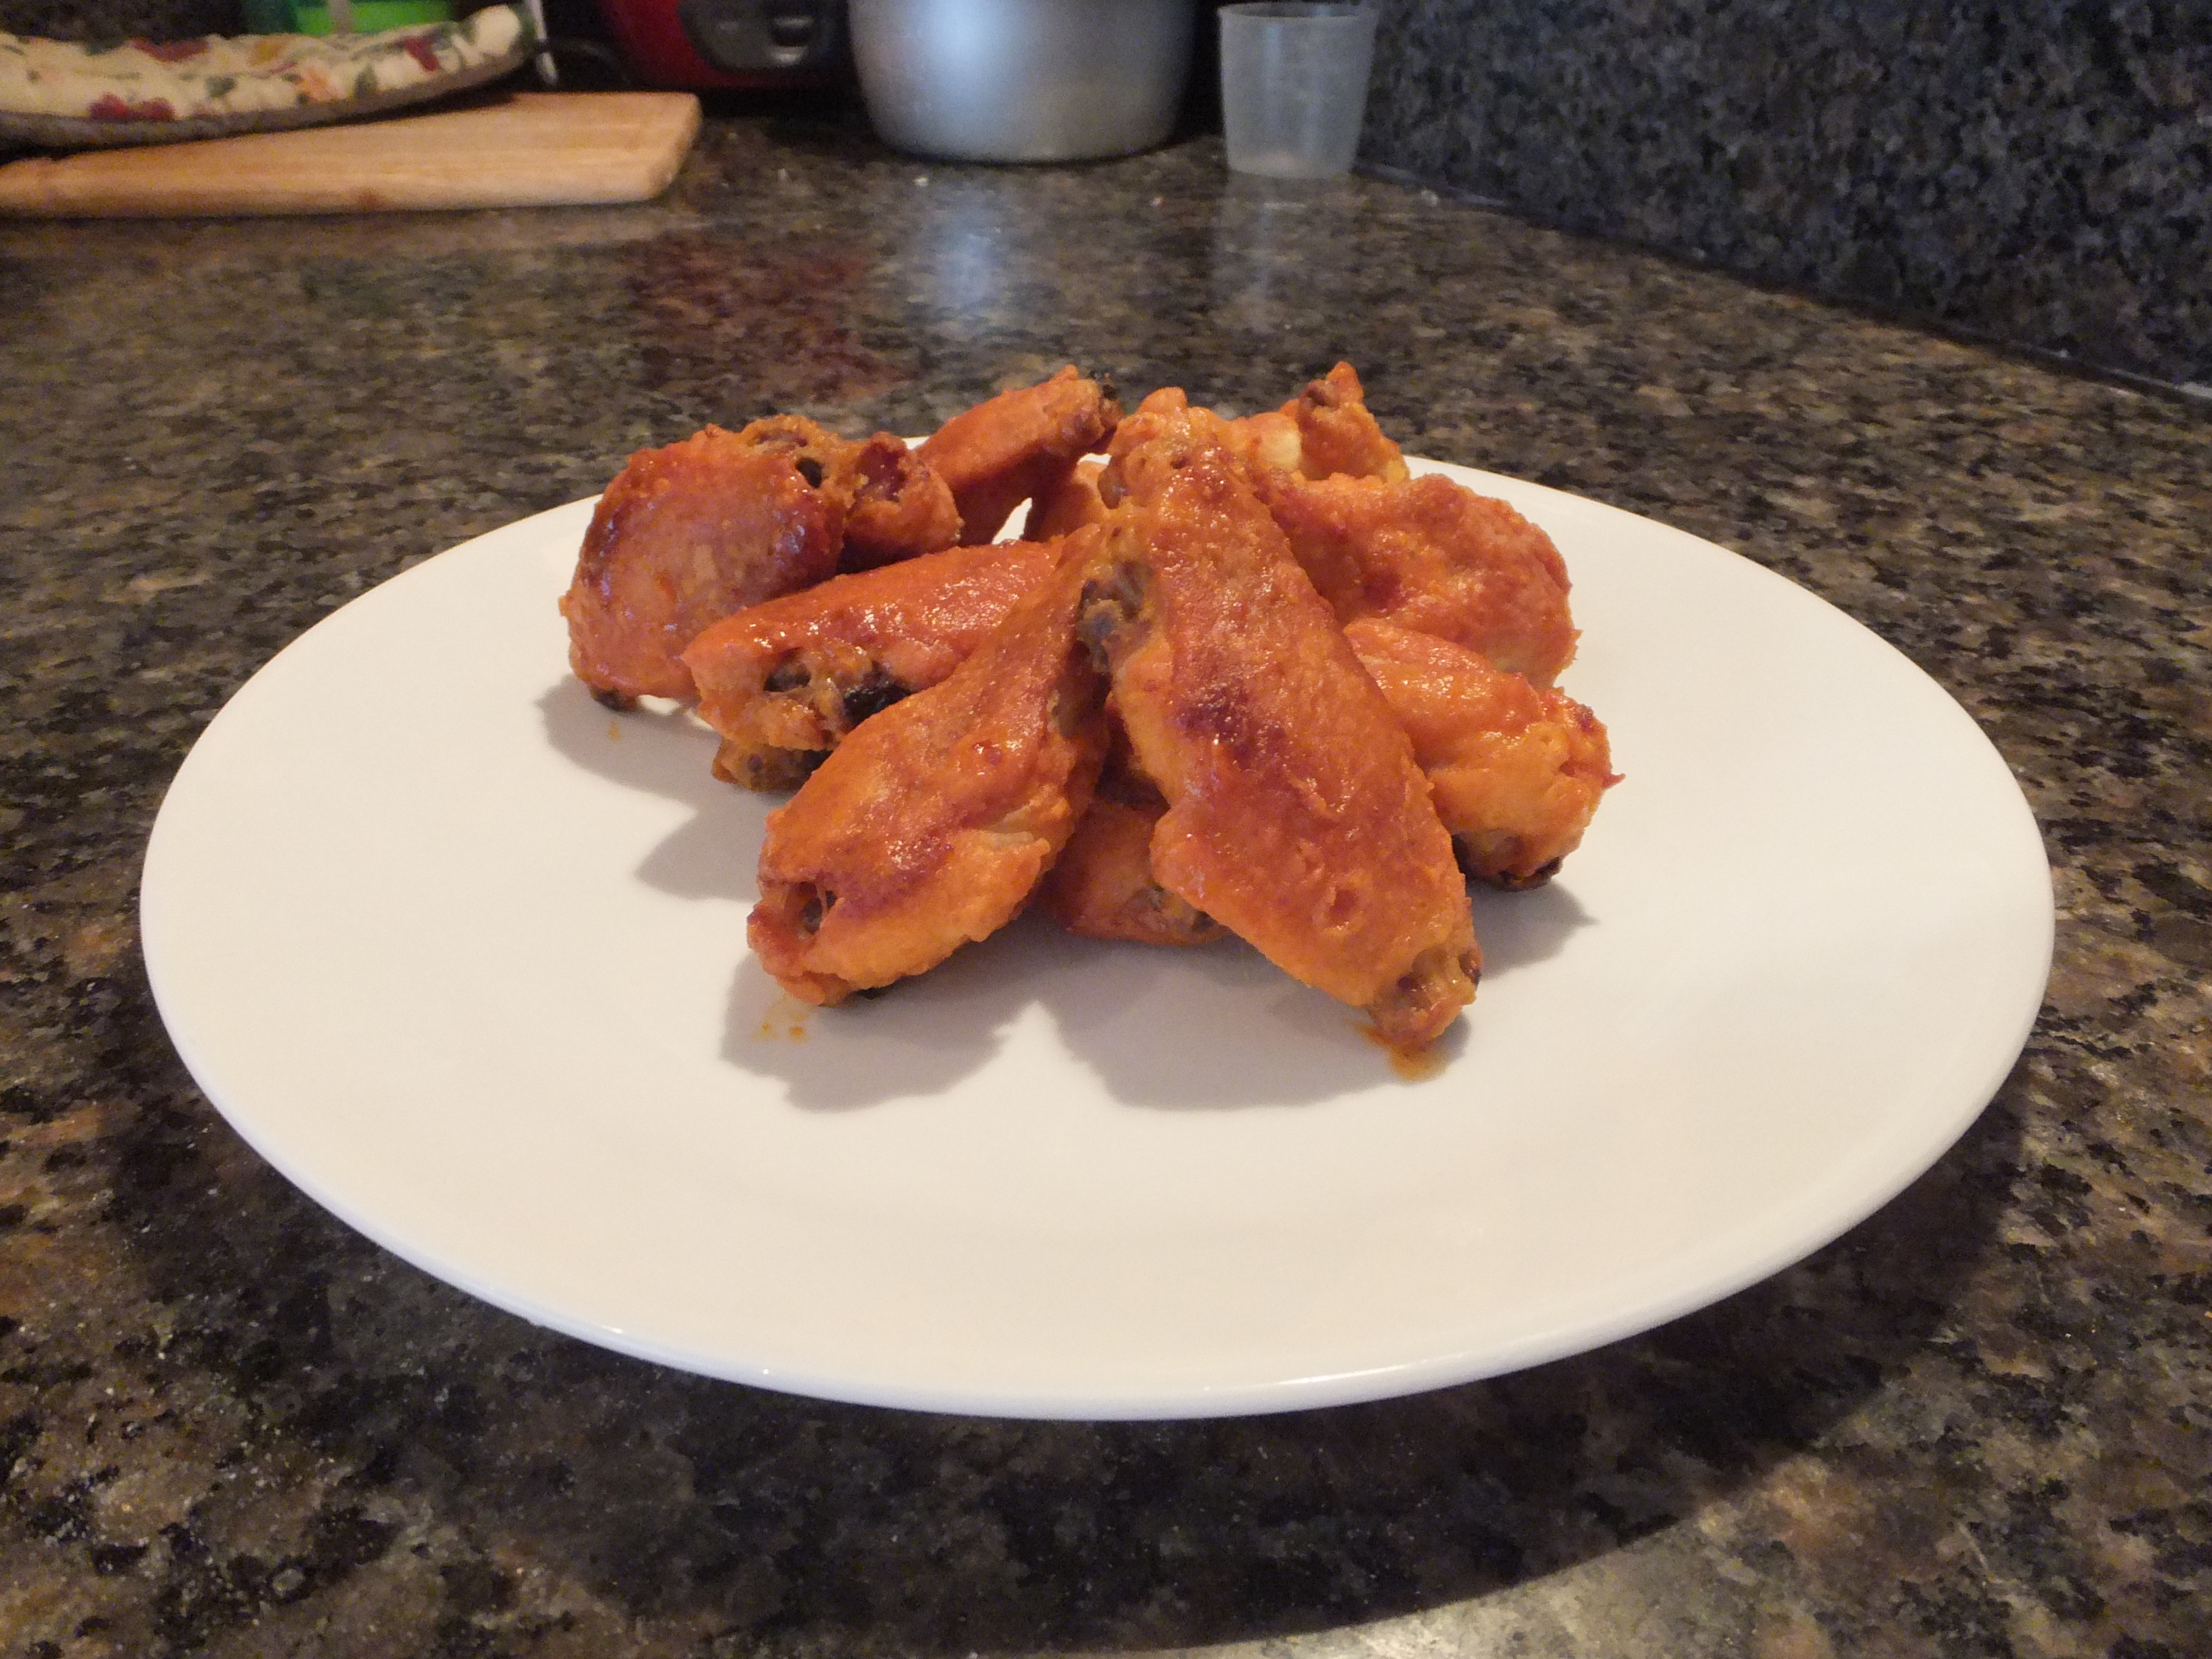
\includegraphics[width=\linewidth,trim=150px 300px 150px 450px, clip=true]{oven_fried_wings-01.jpeg}
    \end{image}
  \end{images}

  \begin{steps}
  \item Trim and seperate the chicken wings
  \item Put the flour in a plastic bag, and then dump the wings in.
    Shake them around.
  \item Grease two half sheet-pans and heat them in a 450\degree F
    oven.
  \item Spread the wings evenly over the heated pans and return them
    to the oven.
  \item Bake for 20 minutes, flip the wings, and bake for another 20
    minutes.
  \end{steps}

  \begin{notes}
  \item You should probably put some sauce on these wings... :)
  \end{notes}
\end{recipe}
\end{document}
